% !TeX spellcheck = fr_FR
\documentclass[../main.tex]{subfiles}

\begin{document}

Un processus ponctuel $N = (N_t)$ compte le nombre d'événements sur $[0,t]$. Le nombre d'événements entre deux instants $s\leq t$ est donc $N_t - N_s$. Si on se donne une filtration $\mathds{F} = (F_t)$ adaptée au processus $N$, il existe un processus prévisible $\lambda$ associé à $N$ appelé \textit{intensité}, vérifiant
\[
	\EE [N_{t+h} - N_t \mid \mathcal{F}_t] \underset{h\to 0}{=} \lambda_th + o(h).
\]
ou succinctement $\EE[dN_t] = \lambda_t\,dt$.
Ainsi, plus l'intensité $\lambda_t$ est élevée, plus la probabilité d'avoir un événement dans l'immédiat est élevée.

Un processus \textit{multivarié} $N$ compte des événements de plusieurs types $k$. Ses composantes $N^k$ ont chacune leur propre intensité $\lambda^k$. Dans la suite, on notera $\bar{\lambda}_t = \sum_{k=1}^{K}\lambda^k_t$ l'intensité totale du processus, pour tous les types d'événements.

On cherche ici à modéliser des \textit{séquences} d'événements ${\{(t_i,k_i)\}}_i$ arrivant à des instants distincts $0<t_1 < \cdots$ et de \textit{type} $k_i$.

Si on se donne un modèle $P = \PP(\,\cdot\,\mid \Theta)$ de la loi de nos séquences d'événements, la probabilité que $I$ événements $t_1<\cdots<t_I$ de types $k_i$ surviennent entre les instants $0$ et $T > 0$ a une log-vraisemblance
\begin{equation}\label{eq:likelihood}
	\mathcal{L} =
	\log P(\{(t_i,k_i)\}_{1\leq i\leq I}) =
	\sum_{i=1}^{I} \log P((t_i,k_i)\mid \mathcal{F}_{t_{i-1}}, t_i)
	+ \log P(t_{I+1}>T\mid \mathcal{F}_{t_{I}})
\end{equation}
où $\mathcal{F}_t = \{ (t_i,k_i)\,:\, t_i \leq t \}$.



\subsection{Modèle de base: le processus de Hawkes}

Le processus de Hawkes est un modèle élémentaire de processus ponctuel dépendant de son propre passé. Pour un processus de Hawkes \textit{linéaire}, le processus d'intensité s'écrit sous la forme (vectorielle)
\begin{equation}
\lambda_t = \mu_t + \int_0^t g(t-s)\,dN_s
\end{equation}
où:\begin{itemize}
	\item $N^i_t$ est le nombre total d'événements de type $i$ (la mesure $dN^i_t$ compte le nombre d'événements entre $t$ et $t+dt$),
	\item $\lambda_t^i$ est l'intensité des événements de type $i$,
	\item $\mu^i_t$ est l'intensité de base des événements de type $i$,
	\item $g(t) \in \RR^{K\times K}$ est le \textit{noyau} d'excitation: le coefficient $g_{ij} \geq 0$ contrôle le degré selon lequel les événements de type $j$ influencent l'arrivée des événements de type $j$, et est causal ($g_{ij} = 0$ sur $(-\infty, 0)$).
\end{itemize}

Des choix courants de noyaux d'excitation sont la forme exponentielle $g(t) = \alpha\beta\exp(-\beta t)$ ou la somme de formes exponentielles $g(t) = \sum_q \alpha_q\beta_q\exp(-\beta_q t)$.

\subsection{Réseaux de neurones récurrents}

Les réseaux de neurones récurrents (\textit{recurrent neural networks}, RNN), sont des modèles de réseaux de neurones avec mémoire, qui prennent en compte l'historique entier de leurs \textit{inputs} au cours de leur entraînement, via état caché $h\in\RR^D$ (\textit{hidden state}), mis à jour à chaque passage dans le réseau. L'entier $D$ est la dimension cachée du réseau. La figure \autoref{fig:simpleRNN} illustre une architecture RNN simple, dite de \citeauthor{elman1990srnn} \cite{elman1990srnn}.

Ces architectures récurrentes se sont montrées particulièrement efficaces dans le domaines de la vision par ordinateur ou de la compréhension de texte, le \textit{natural language processing} (NLP). \cite{unreasonableEffectivenessRNN}

\begin{figure}[!ht]
	\centering
	\includegraphics[height=0.2\textheight]{diagrams/rnn.pdf}
	\caption{Les architectures RNN impliquent l'usage de boucles: la sortie $h_t$ est utilisée calculer $h_{t+1}$.}\label{fig:simpleRNN}
\end{figure}

Il s'agit ici de modéliser des événements auxquels sont associés à la fois des types mais aussi des temps d'arrivée qui se répartissent en temps continu et peuvent refléter des phénomènes de relaxation ou d'excitation. Une façon de faire est de considérer que l'intensité du processus est modélisée par un réseau de neurones récurrent:
\[
	\lambda_t = \phi(t\mid \mathcal{F}_t)
\]
où l'architecture récurrente permet au réseau $\phi$ de dépendre de l'information $\mathcal{F}_t$ que l'on détient sur le passé: temps d'arrivée des événements et types de ces derniers.



\subsubsection{Réseau récurrent avec amortissement (Decay-RNN)}\label{sssec:decayRNN}

On postule que l'intensité est non-linéaire de la forme
\begin{equation}\label{eq:decayRNNintensity}
\lambda_t = f(W_l h(t))
\end{equation}
où $h(t)\in\RR^D$ est un état caché en temps continu. Il s'agit d'une variante des architectures récurrentes standard de \citeauthor{elman1990srnn} introduisant un amortissement exponentiel de l'état caché $h(t)$ pour prendre en compte le temps. C'est inspiré de ce que font \citeauthor{meiEisnerNeuralHawkes} \cite{meiEisnerNeuralHawkes}.

Le réseau prend en entrée l'intervalle de temps $\Delta t_i$ entre deux événements et le type $k_i\in\llbracket 1,K\rrbracket$, transformé en vecteur $x_i\in\RR^K$ en utilisant un \textit{embedding}.
Le temps écoulé depuis un événement en $t_{i-1}$ est pris en compte en amortissant l'état caché
\begin{equation}
h(t) = h_{i}e^{-\delta_i(t-t_{i-1})},\quad t\in(t_{i-1},t_i]
\end{equation}
où les paramètres $h_i$ et $\delta_i$ sont mis à jour pour l'intervalle $(t_i,t_{i+1}]$ via les équations
\begin{subequations}
\begin{align}
	h_{i+1} &= \tanh(W_{hh}h(t_i) + W_{xh}x_i + b_{h})\quad\text{(\textit{hidden layer})} \\
	\delta_{i+1} &= f(W_{hd}h(t_i) + W_{xd}x_i + b_d).
\end{align}
\end{subequations}

La fonction d'activation $f$ utilisée est la <<~Softplus~>>
\[
	x\mapsto \frac{1}{\beta}\log(1+e^{\beta x}),\quad\beta > 0,
\]
une approximation régulière et strictement positive de la fonction ReLU $x\mapsto \max(x,0)$. Cela garantit que $\lambda_t > 0$.

La valeur de $h(t)$ peut signaler un comportement inhibiteur pour certaines composantes (valeur proche de $-1$) et excitateur pour d'autres (valeur proche de $1$), qui est d'autant plus fort que le dernier événement est récent. L'état caché est ramené vers $0$ sur les temps longs, mais dernière couche transforme l'état caché $h(t)$ en une somme d'exponentielles, ce qui permet d'accéder à une classe assez large de dynamiques: un effet excitateur dominant pour l'une des composantes du processus peut s'affaiblir ou même laisser la place à un effet inhibiteur. La \autoref{fig:exampleRNNIntensityTraj} montre quelques dynamiques possibles.

\begin{figure}[!ht]
	\begin{subfigure}{\linewidth}
		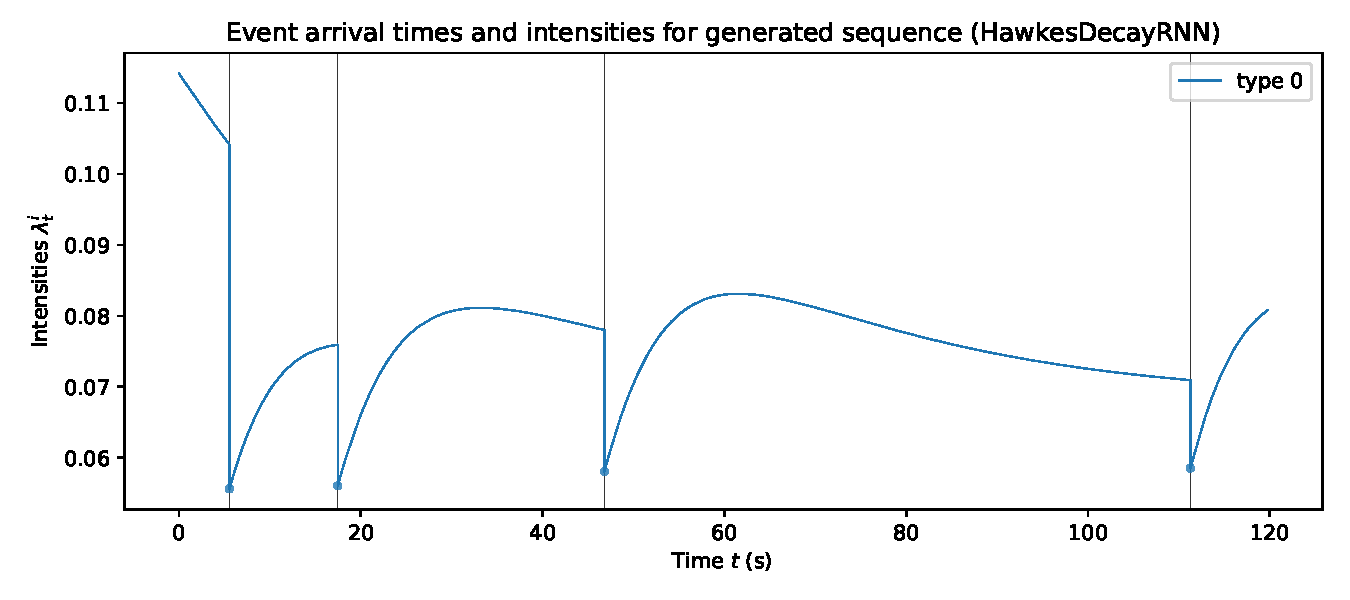
\includegraphics[width=\linewidth]{../notebooks/example_rnnplot.pdf}
		\caption{Réalisation d'un processus RNN avec amortissement univarié. Il présente une dynamique auto-excitatrice semblable à un Hawkes à noyau exponentiel.}
	\end{subfigure}
	\begin{subfigure}{\linewidth}
		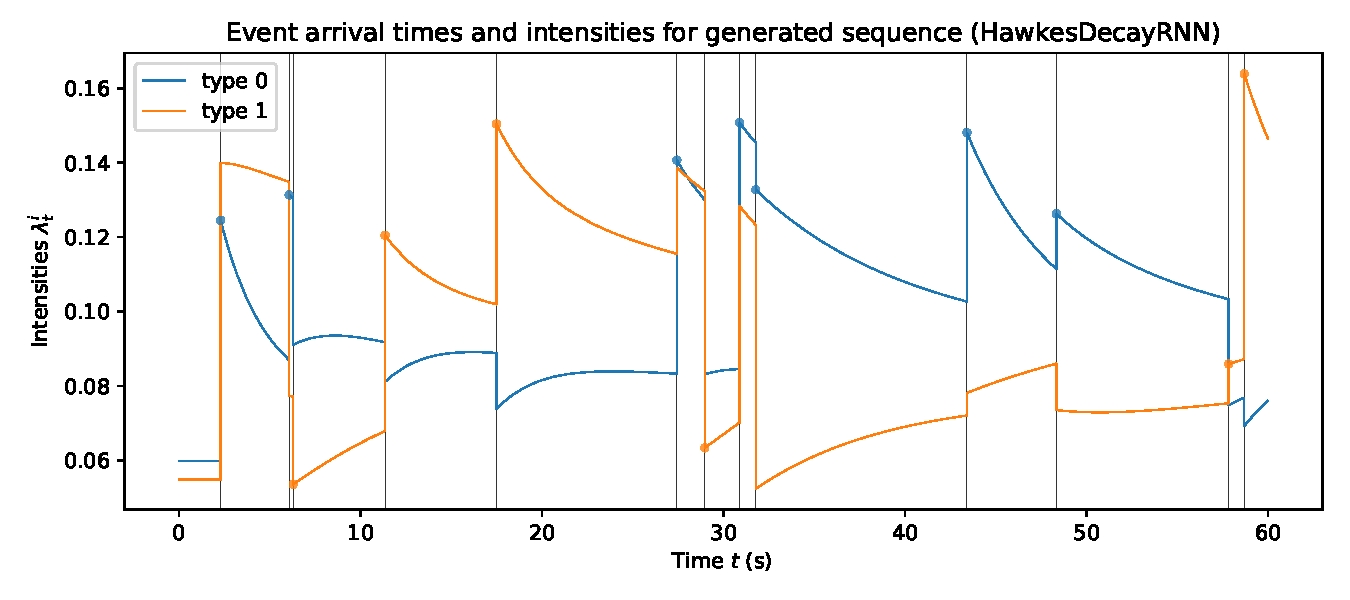
\includegraphics[width=\linewidth]{../notebooks/example_rnnplot2d.pdf}
		\caption{Réalisation d'un Decay-RNN bivarié. Il présente des effets d'excitation-inhibition mutuels ou auto-suscités.}
	\end{subfigure}
	\caption{Trajectoires d'intensité et événements pour des processus Decay-RNN univarié et bivarié, à poids aléatoires.}\label{fig:exampleRNNIntensityTraj}
\end{figure}


\subsubsection{Réseau LSTM avec amortissement}

\citeauthor{meiEisnerNeuralHawkes} proposent en fait d'utiliser une architecture inspirée des réseaux <<~\textit{Long Short-Term Memory}~>> (LSTM). Ces réseaux récurrents plus complexes permettent un contrôle plus fin de l'information qui reste en mémoire.

L'intensité est définie à partir de l'état caché $h(t)$ comme dans \eqref{eq:decayRNNintensity}, et cet état caché est lié à un état-cellule $c(t)$ (\textit{cell state}) en temps continu par la relation usuelle des réseaux LSTM
\begin{equation}
	h(t) = o_i \odot \tanh(c(t)).
\end{equation}

L'état-cellule $c(t)$ suit une évolution exponentielle entre deux événements $t_{i-1}$ et $t_i$:
\begin{equation}\label{eq:ctlstmCellState}
c(t) = \bar{c}_{i} + (c_{i} - \bar{c}_{i})e^{-\delta_i (t - t_{i-1})},\quad t\in(t_{i-1}, t_{i}].
\end{equation}
Les paramètres sont mis à jour pour l'intervalle $(t_i, t_{i+1}]$ via les équations:
\begin{subequations}
\begin{align}
	\mathrm{i}_{i+1} &= \sigma(W_{h\mathrm{i}}h(t_i) + W_{x\mathrm{i}}x_i + b_{\mathrm{i}}) \\
	f_{i+1} &= \sigma(W_{hf}h(t_i) + W_{xf}x_i + b_{f}) \\
	\bar{\imath}_{i+1} &= \sigma(W_{h\bar{\imath}}h(t_i) + W_{x\bar{\imath}}x_i + b_{\bar{\imath}}) \\
	\bar{f}_{i+1} &= \sigma(W_{h\bar{f}}h(t_i) + W_{x\bar{f}}x_i + b_{\bar{f}}) \\
	z_{i+1} &= \tanh(W_{hz}h(t_i) + W_{xz}x_i + b_{z}) \\
	\delta_{i+1} &= f(W_{hd}x_i + W_{xd}h(t_i) + b_d) \\
	c_{i+1} &= f_{i+1}\odot c(t_i) + \mathrm{i}_{i+1}\odot z_{i+1} \\
	\bar{c}_{i+1} &= \bar{f}_{i+1}\odot \bar{c}_i + \bar{\imath}_{i+1}\odot z_{i+1} \\
	o_{i+1} &= \sigma(W_{ho}h(t_i) + W_{xo}x_i + b_o)
\end{align}
\end{subequations}

\begin{figure}[!h]
	\begin{subfigure}{\linewidth}
		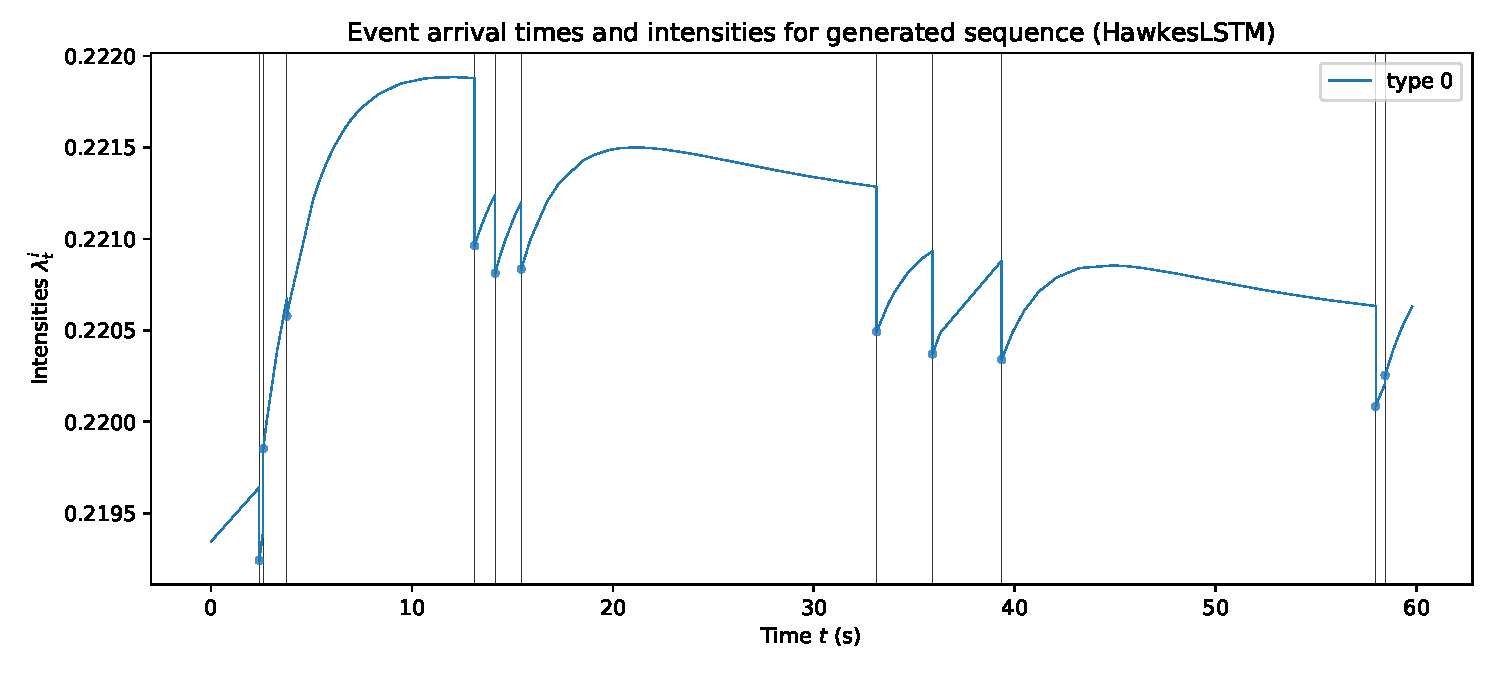
\includegraphics[width=\linewidth]{../notebooks/example_lstmplot.pdf}
	\end{subfigure}
	\begin{subfigure}{\linewidth}
		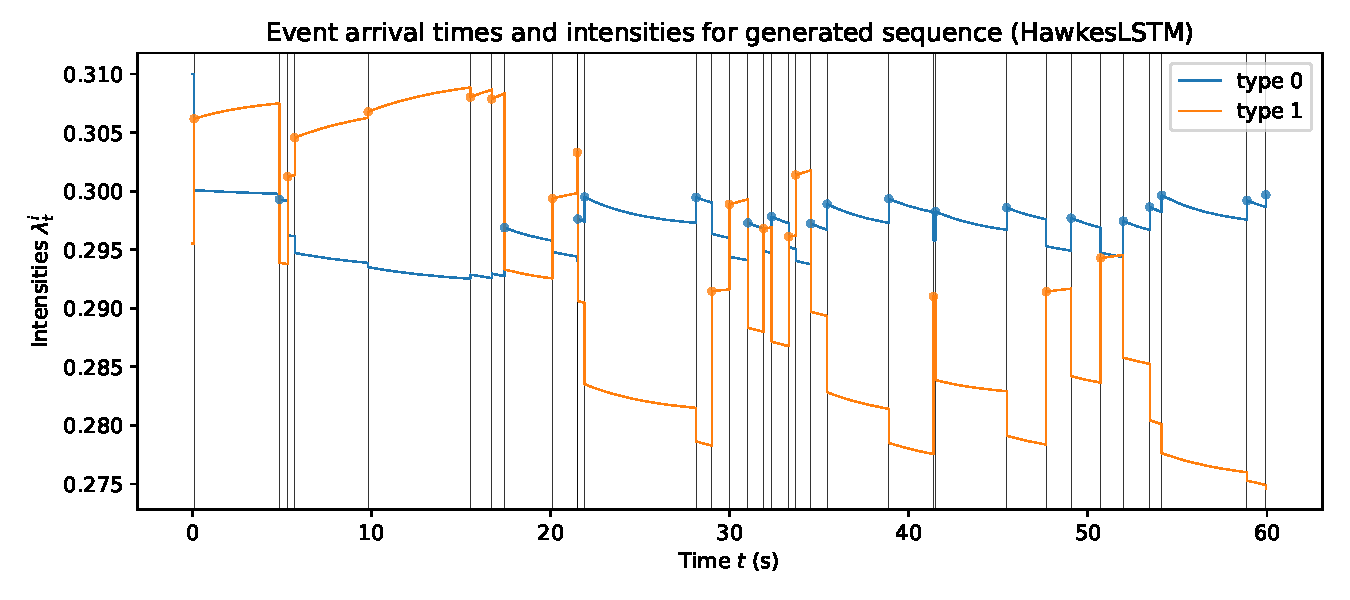
\includegraphics[width=\linewidth]{../notebooks/example_lstmplot2d.pdf}
	\end{subfigure}
	\caption{Trajectoires générées par un modèle LSTM non-entraîné, avec des poids générés aléatoirement.}\label{fig:exampleLSTMIntensityTraj}
\end{figure}

Ce réseau offre également une dynamique riche comme le modèle Decay-RNN. \citeauthor{meiEisnerNeuralHawkes} introduisent une valeur de long terme $\bar{c}_i$ pour l'état-cellule. La \autoref{fig:exampleLSTMIntensityTraj} illustre un cas unidimensionnel où chaque événement a un effet auto-inhibiteur immédiat, qui est corrigé par une excitation externe qui s'affaiblit.




\end{document}